\chapter{Arkitektur}

%% indledning til kapitel skal være her...

% Her beskrives systemets overordnede systemarkitektur. Her anvendes SysML til beskrivelse af struktur og interaktion imellem komponenterne. Fastlæggelse af grænseflader mellem systemets komponenter og beskrivelse af disse er vigtigt.
\lipsum[2]

\section{4 + 1}\todo{find better name?}

\subsection{User-story view}

\subsection{Logical view}

\subsection{Implementation view} % også kendt som development view

\subsection{Process view}
Dette view beskriver systemets concurrency. Systemet håndterer at flere typer platforme kan tilgå serveren og modtage data på samme tid. Dette fremgår af Figur~\ref{fig:processview}
\begin{figure}
	\centering
	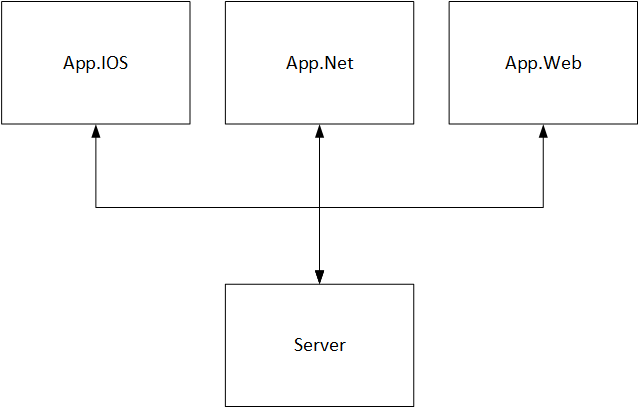
\includegraphics[width=0.7\linewidth]{figs/arkitektur/Processview.png}
	\caption{Process view}
	\label{fig:processview}
\end{figure}

\subsection{Deployment view} % muligvis ikke nødvendig

